\documentclass{standalone}
\usepackage{tikz}
\usetikzlibrary{shapes,arrows}

\begin{document}

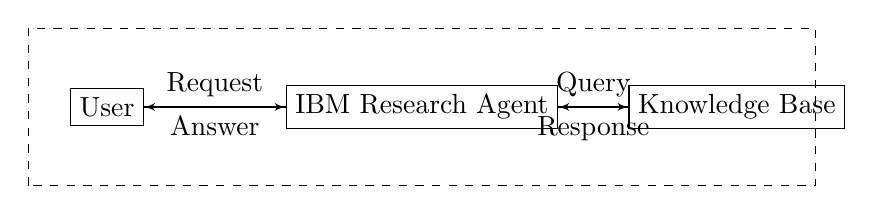
\begin{tikzpicture}[auto,node distance=2cm,>=latex']
  % Define nodes
  \node [draw, rectangle] (user) at (0,0) {User};
  \node [draw, rectangle] (agent) at (4,0) {IBM Research Agent};
  \node [draw, rectangle] (knowledge) at (8,0) {Knowledge Base};

  % Draw arrows between nodes
  \draw[->] (user) -- node {Request} (agent);
  \draw[->] (agent) -- node {Query} (knowledge);
  \draw[->] (knowledge) -- node {Response} (agent);
  \draw[->] (agent) -- node {Answer} (user);

  % Optional: add some decorations
  \draw[dashed] (-1,-1) rectangle (9,1); % bounding box
\end{tikzpicture}

\end{document}